\section{Auswertung}
\label{sec:Auswertung}

%Siehe \autoref{fig:plot}!
\subsection{Verzögerungszeit}
Im folgenden wird für Messgrößen die eine Anzahl beschreiben, eine Poisson-verteilte Messunsicherheit $\sigma = \sqrt{N}$ angenommen.
In weiteren Rechnungen wird mithilfe der Python-Bibliothek \textit{uncertainties}\cite{uncertainties} die Fehlerfortpflanzung durchgeführt.
\\
Bevor die Messung zur Bestimmung der Lebensdauer der Myonen beginnen kann, muss die Apparatur justiert und kalibriert werden.
Die Verzögerungsleitungen werden jeweils für einen Photomultiplier systematisch untersucht.
In einem Zeitraum von $\qty{10}{\second}$ wird die Anzahl Impulse $N$ für eine definierte Verzögerungszeit $t$ aufgenommen.
Die gemessenen Impulse $N$ bei eingestellter Verzögerungszeit $t$ sind in \autoref{tab:verzoegerung} aufgelistet.
Eine Verzögerung auf der linken bzw. rechten Leitung entspricht einer negativen bzw. positiven Verzögerungszeit.
\begin{table}
    \centering
    \caption{Die Anzahl detektierter Ereignisse $N$ in Abhängigkeit der eingestellten Verzögerungszeit $t$ der Verzögerungsleitungen.
    Eine Verzögerung auf der linken bzw. rechten Leitung entspricht einer negativen bzw. positiven Verzögerungszeit.
    Die Messzeit beträgt jeweils $\qty{10}{\second}$.
    }
    \label{tab:verzoegerung}
    \begin{tabular}{cc|cc}
        \toprule
        $t \,/\, \unit{\nano\second}$ & Anzahl Impulse $N$ in $\qty{10}{\second}$ & $t \,/\, \unit{\nano\second}$ & Anzahl Impulse $N$ in $\qty{10}{\second}$ \\
        \midrule
        -28 & 0 & 1 & 215 \\
        -26 & 0 & 2 & 227 \\
        -24 & 0 & 3 & 237 \\
        -22 & 0 & 4 & 260 \\
        -20 & 1 & 6 & 281 \\
        -18 & 9 & 8 & 300 \\
        -16 & 10 & 10 & 255 \\
        -14 & 23 & 12 & 234 \\
        -12 & 35 & 14 & 162 \\
        -10 & 57 & 16 & 96 \\
        -8 & 99 & 18 & 75 \\
        -6 & 168 & 20 & 45 \\
        -4 & 183 & 22 & 25 \\
        -3 & 188 & 24 & 20 \\
        -2 & 205 & 26 & 10 \\
        -1 & 221 & 28 & 6 \\
        0 & 212 & & \\
        \bottomrule
    \end{tabular}
\end{table}
\begin{figure}
    \centering
    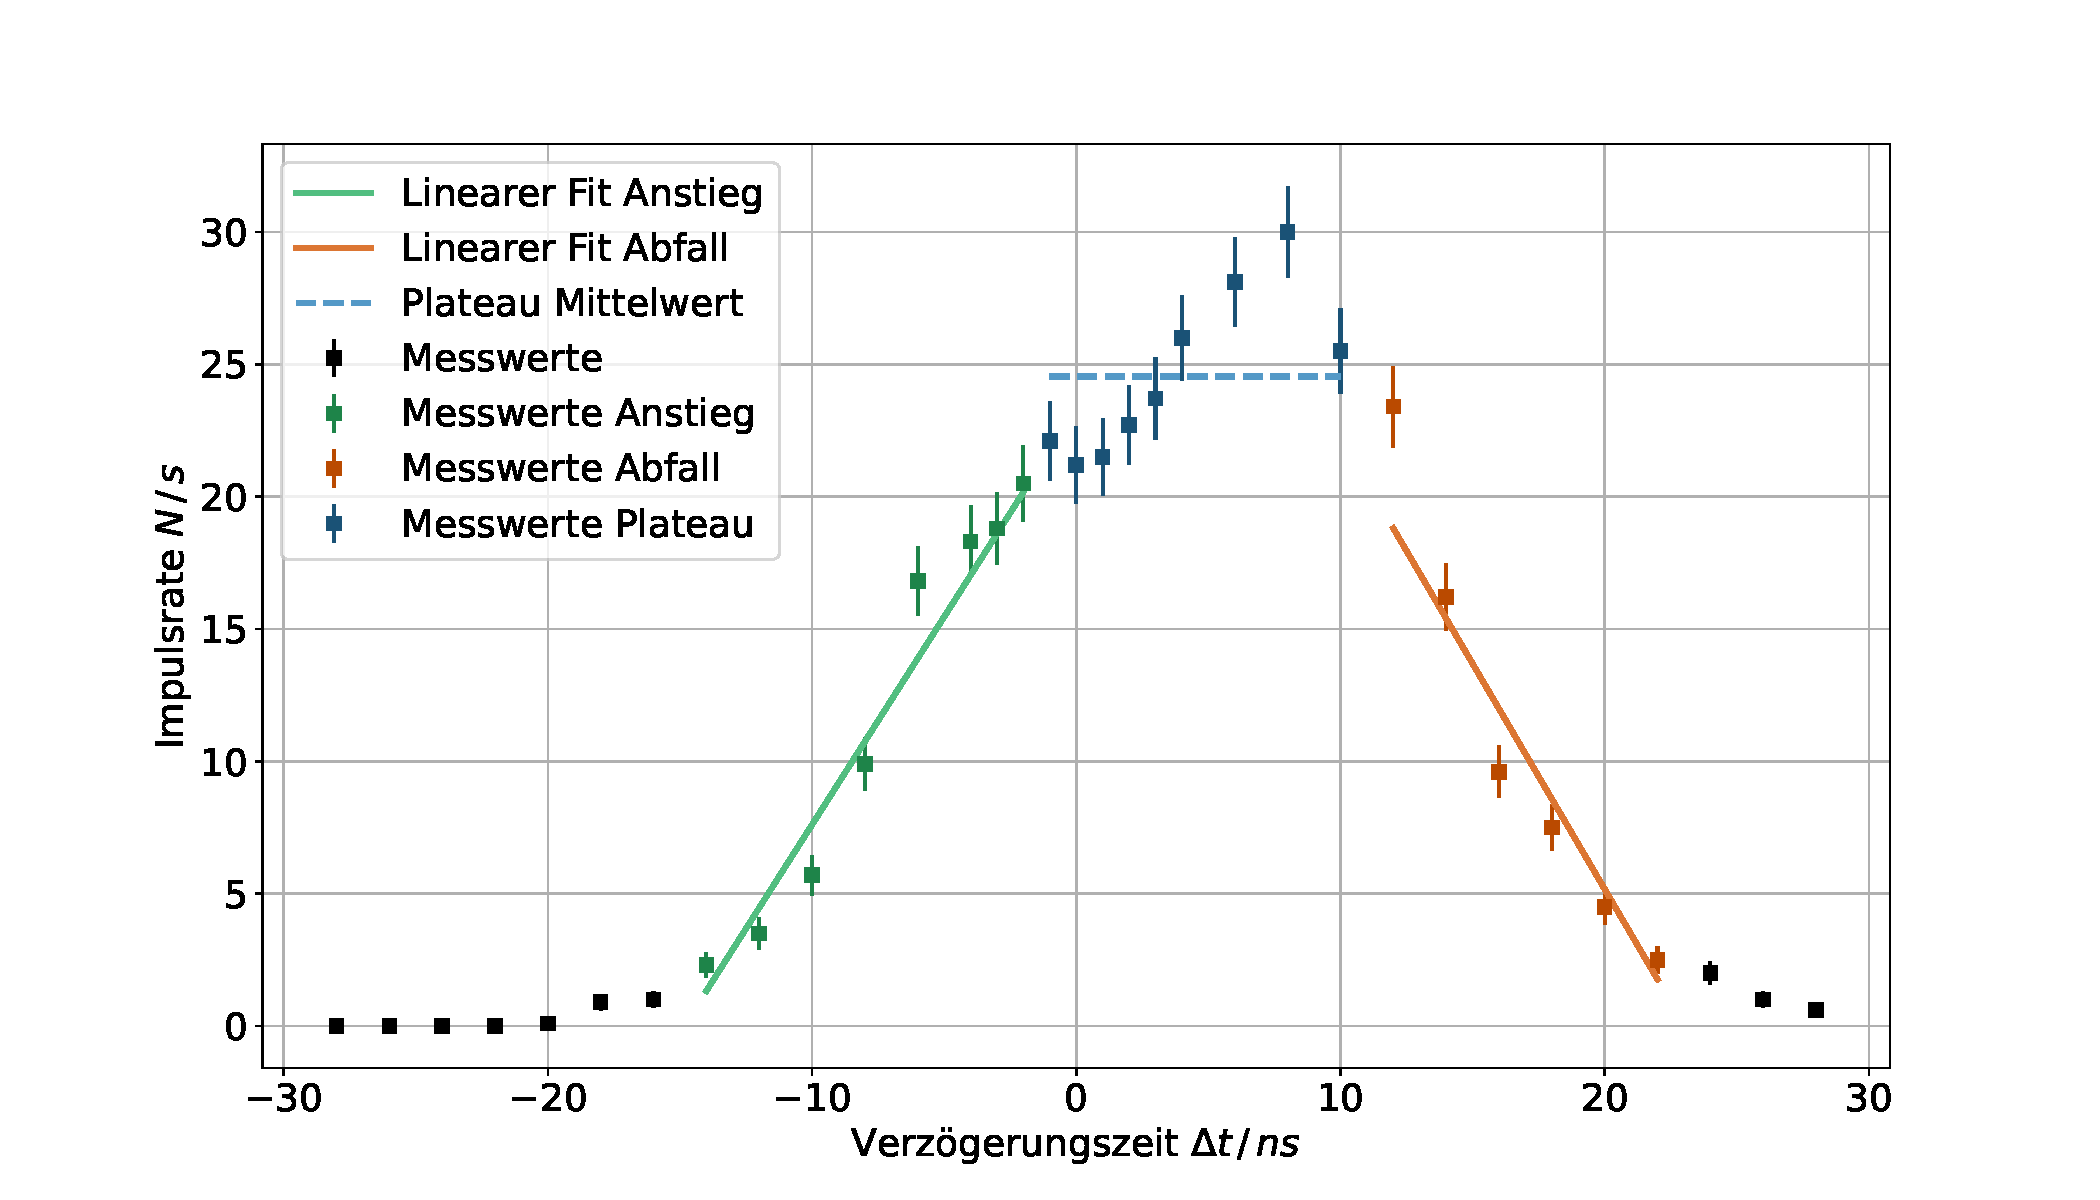
\includegraphics[width=0.95\textwidth]{content/plots/verzoegerungszeit.pdf}
    \caption{Die gemessene Ereignisrate $N$ in Abhängigkeit der Verzögerungszeit $\Delta t$.
    Die Messwerte werden in 3 Bereiche unterteilt, wobei die ersten und lette
    Der Anstieg und Abfall wird näherungsweise jeweils durch einen linearen Fit dargestellt.
    Das Mittel über die zum Plateau zugehörigen Messwerte definiert die Plateau-Höhe.}
    \label{fig:verzoegerung}
\end{figure}
Die Messwerte werden in einen Anstiegs-, Aufstiegs- und Plateau-Bereich unterteilt.
Statt die Gesamtanzahl gemessener Impulse in einem bestimmten Zeitraum wird die Impulsrate pro Sekunde betrachtet.
Im Mittel ergibt sich eine Plateau-Höhe von
\begin{equation}
    N_\text{Plateau} = \qty{24.53(103)}{\frac{1}{\second}} \,.
\end{equation}
Für den Anstiegs- und Abstiegsbereich wird ein linearer Fit der Form
\begin{equation*}
    N = a \cdot t + b
\end{equation*}
mithilfe der Methode der kleinsten Quadrate (\textit{scipy.optimize.curve\_fit}\cite{scipy}) durchgeführt.
Aus der Ausgleichsrechnung folgen die Parameter
\begin{align*}
    a_\text{Anstieg} &= \qty{1.57(14)}{\frac{1}{\nano\second^2}},\qquad b_\text{Anstieg} = \qty{23.31(159)}{\nano\second}, \\
    a_\text{Abfall} &= \qty{-170(25)}{\frac{1}{\nano\second^2}},\qquad b_\text{Abfall} = \qty{39.25(480)}{\nano\second} \,.
\end{align*}
Aus den Schnittpunkten der Ausgleichsgeraden mit der halben Plateau-Höhe
\begin{align*}
    t_\text{Anstieg} &= \qty{-7.03(124)}{\nano\second} \\
    t_\text{Abfall} &= \qty{15.84(363)}{\nano\second}
\end{align*}
kann die Halbwertsbreite als Differenz der Schnittpunkte zu
\begin{equation}
    \Delta t = t_\text{Abfall} - t_\text{Anstieg} = \qty{22.87(386)}{\nano\second}
\end{equation}
bestimmt werden.
Die Messwerte, Plateau-Höhe und Ausgleichsgeraden sind in \autoref{fig:verzoegerung} dargestellt.
Um im Folgenden eine möglichst hohe Impulsrate zu messen, wird die Verzögerungszeit auf $\Delta t = \qty{8}{\nano\second}$ eingestellt.%???
\FloatBarrier

\subsection{Kalibration des Vielkanalanalysators}
Der Vielkanalanalysator ordnet ein Ereignis einem Kanal zu.
Jeder Kanal deckt ein definiertes Zeitintervall ab.
Die mittlere Zeit jedes Kanals wird mithilfe eines Impulsgenerators bestimmt.
\\
Die ermittelten Kanäle für bestimmte eingestellte Impulsdauern am Generator sind in \autoref{tab:kalibration} gelistet.
\begin{table}
    \centering
    \caption{Die ermittelten Kanäle am Vielkanalanalysator in Abhängigkeit der eingestellten Impulsdauer am Impulsgenerator.}
    \label{tab:kalibration}
    \begin{tabular}{cc}
        \toprule
        $t \,/\, \unit{\micro\second}$ & Kanal \\
        \midrule
        0.5 & 4 \\
        1 & 16 \\
        2 & 38 \\
        3 & 61 \\
        4 & 84 \\
        5 & 107 \\
        6 & 129 \\
        7 & 152 \\
        8 & 175 \\
        9 & 197 \\
        9.9 & 218 \\
        \bottomrule
    \end{tabular}
\end{table}
Die Kanäle sind mit der Impulsdauer linear korreliert.
Ein linearer Fit der Form
\begin{equation*}
    t = a \cdot ch + b
\end{equation*}
wird durchgeführt, wobei $ch$ die Kanäle ("`channel"') im Bereich $[0, 511]$ und $t$ die Impulsdauer beschreibt.
Die Ausgleichsgerade mit den Parametern
\begin{align*}
    a_\text{Kalibration} = \qty{0.0440(00001)}{\frac{1}{\second}}, \qquad b_\text{Kalibration} = \qty{0.3125(00079)}{}
\end{align*}
und die Messwerte sind \autoref{fig:kalibration} abgebildet.
\begin{figure}
    \centering
    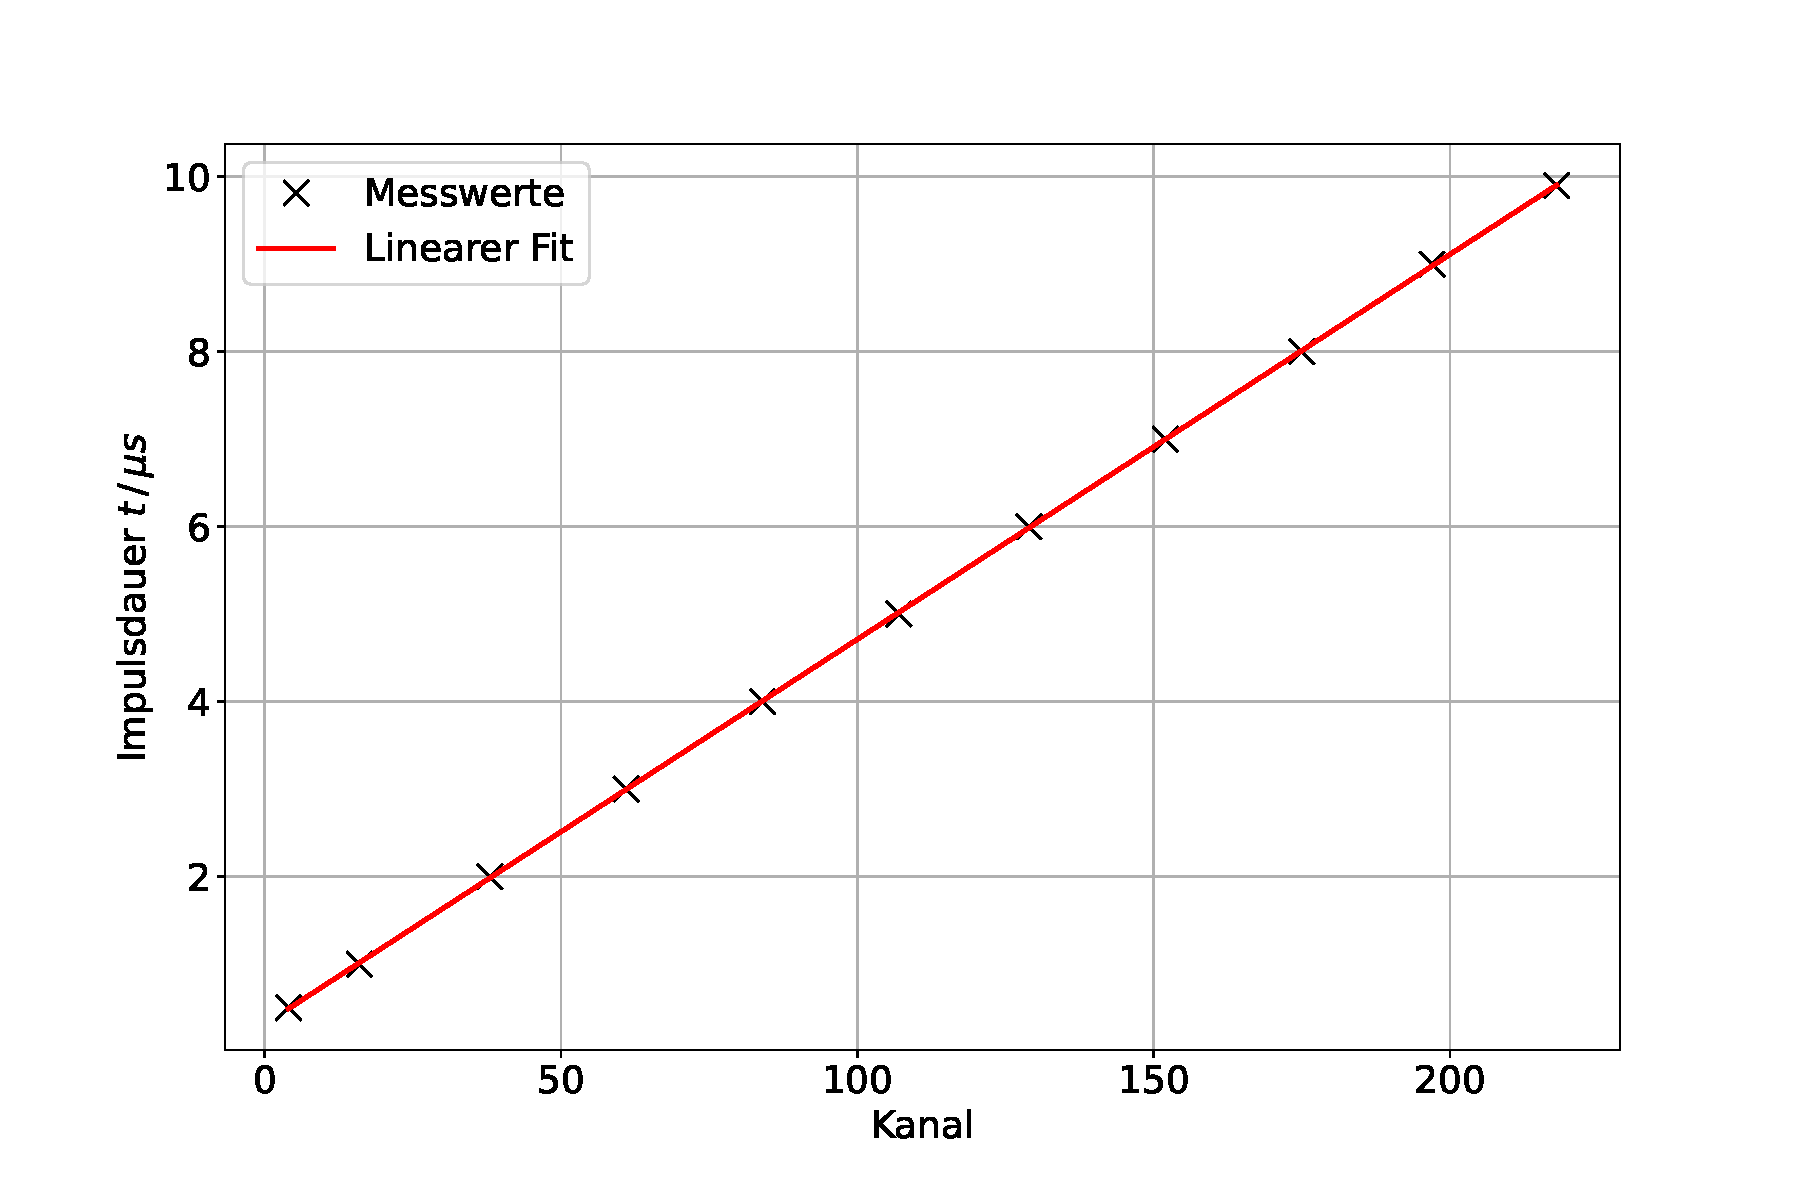
\includegraphics[width=0.9\textwidth]{content/plots/calibration.pdf}
    \caption{Die ermittelten Kanäle des Vielkanalanalysators in Abhängigkeit der eingestellten Impulsdauer.
    Ein linearer Fit verdeutlicht die starke lineare Korrelation zwischen den Variablen.
    }
    \label{fig:kalibration}
\end{figure}
Jedem Kanal kann jetzt eine Zeit zugeordnet werden.
\FloatBarrier

\subsection{Statistische Abschätzung der Untergrundereignisse}
Die eigentliche Messung der Lebensdauer der Myonen umfasst eine Messzeit von
\begin{equation*}
    t_\text{mess} = \qty{158234}{\second} \,.
\end{equation*}
Die Gesamtanzahl der Start- $N_\text{Start}$ und Stopsignale $N_\text{Stop}$ beträgt
\begin{align*}
    N_\text{Start} &= \qty{4509112(2123)}{}, \\
    N_\text{Stop} &= \qty{17526(132)}{} \,.
\end{align*}
Durch ein eintreffendes Myon wird das Startsignal ausgelöst.
Zerfällt das Myon in der Suchzeit $T_S = \qty{10}{\micro\second}$ wird ein weiteres Signal, das Stopsignal detektiert.
Im Folgenden wird die Untergrundrate mit statistischen Methoden abgeschätzt.
Die Ereignisrate beträgt im Durchschnitt etwa $n = \qty{28.5}{\frac{1}{\second}}$.
Die Wahrscheinlichkeit, dass während der Suchzeit $T_S$ ein weiteres Myon in den Detektor trifft folgt einer Poisson-Verteilung.  
Der Untergrund wird mittels \autoref{eqn:} auf %REF???
\begin{equation}
    N_\text{Untergrund,1} = \qty{1283(1)}{}
\end{equation}
abgeschätzt.
Dabei verteilt sich der Untergrund auf alle Kanäle.
\FloatBarrier

\subsection{Experimentell bestimmte Untergrundrate und Lebensdauer der Myonen}
- nur Bins ungleich 0
- kanäle mittels ausgleichgerade in zeit umrechnen
- exp. fit

\begin{figure}
    \centering
    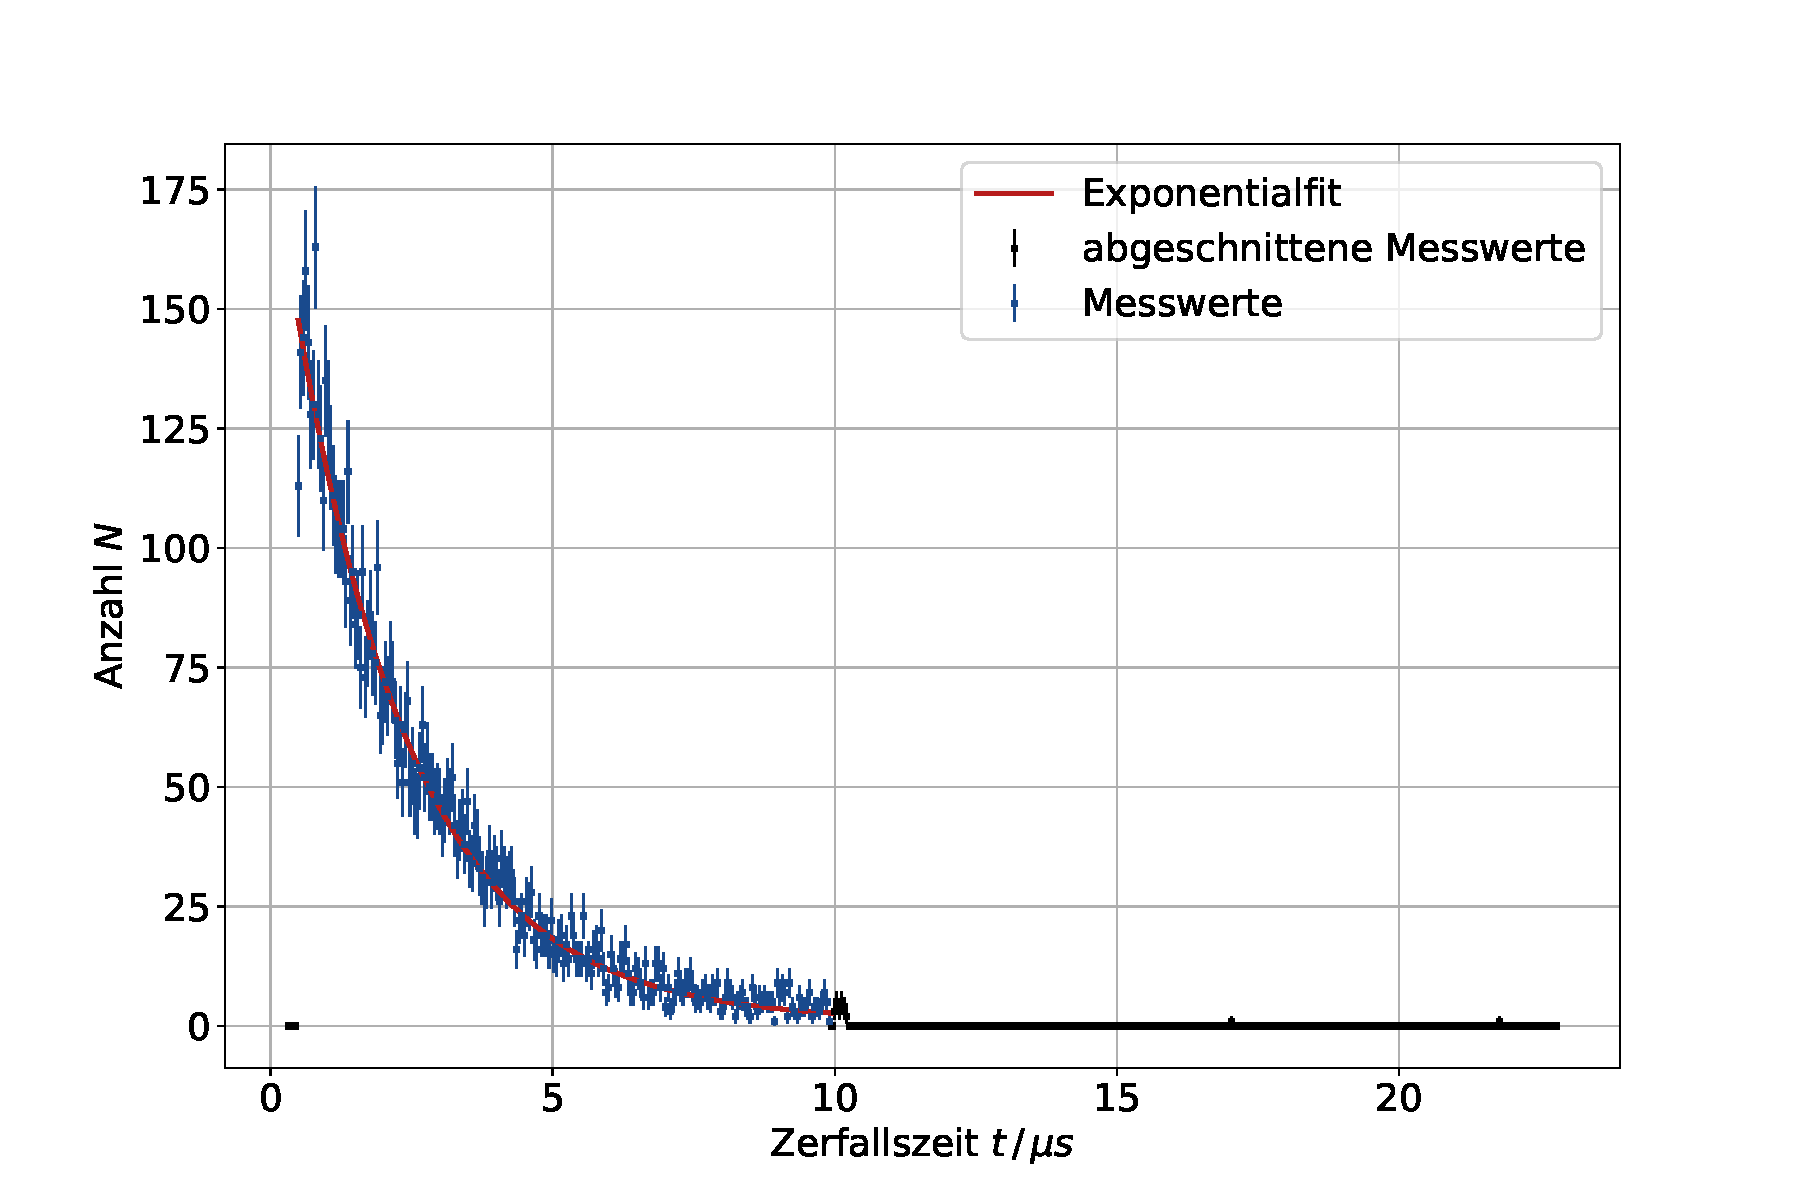
\includegraphics[width=0.9\textwidth]{content/plots/lifetime.pdf}
    \caption{Die Anzahl detektierter Ereignisse $N$ die ein Start- und Stopsignal ausgelöst haben in Abhängigkeit der gemessenen Zerfallszeit $t$.
    Die exponentielle Ausgleichskurve führt direkt zur Lebensdauer der kosmischen Myonen.
    }
    \label{fig:lebensdauer}
\end{figure}